% Created by tikzDevice version 0.12.3.1 on 2021-12-04 18:44:17
% !TEX encoding = UTF-8 Unicode
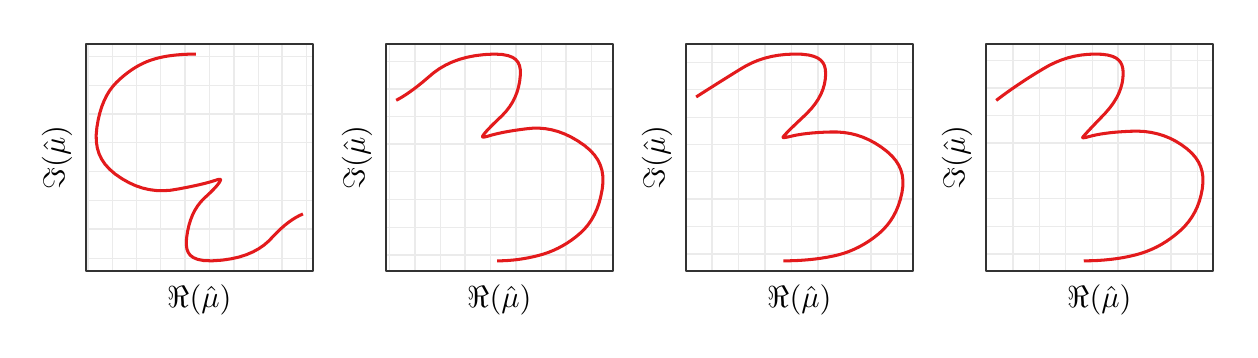
\begin{tikzpicture}[x=1pt,y=1pt]
\definecolor{fillColor}{RGB}{255,255,255}
\begin{scope}
\definecolor{drawColor}{RGB}{255,255,255}
\definecolor{fillColor}{RGB}{255,255,255}

\path[draw=drawColor,line width= 0.6pt,line join=round,line cap=round,fill=fillColor] ( -0.00,  0.00) rectangle (108.41,108.41);
\end{scope}
\begin{scope}
\definecolor{fillColor}{RGB}{255,255,255}

\path[fill=fillColor] ( 20.71, 20.71) rectangle (102.91,102.91);
\definecolor{drawColor}{gray}{0.92}

\path[draw=drawColor,line width= 0.3pt,line join=round] ( 20.71, 25.50) --
	(102.91, 25.50);

\path[draw=drawColor,line width= 0.3pt,line join=round] ( 20.71, 46.29) --
	(102.91, 46.29);

\path[draw=drawColor,line width= 0.3pt,line join=round] ( 20.71, 67.07) --
	(102.91, 67.07);

\path[draw=drawColor,line width= 0.3pt,line join=round] ( 20.71, 87.86) --
	(102.91, 87.86);

\path[draw=drawColor,line width= 0.3pt,line join=round] ( 30.22, 20.71) --
	( 30.22,102.91);

\path[draw=drawColor,line width= 0.3pt,line join=round] ( 47.79, 20.71) --
	( 47.79,102.91);

\path[draw=drawColor,line width= 0.3pt,line join=round] ( 65.36, 20.71) --
	( 65.36,102.91);

\path[draw=drawColor,line width= 0.3pt,line join=round] ( 82.93, 20.71) --
	( 82.93,102.91);

\path[draw=drawColor,line width= 0.3pt,line join=round] (100.50, 20.71) --
	(100.50,102.91);

\path[draw=drawColor,line width= 0.6pt,line join=round] ( 20.71, 35.89) --
	(102.91, 35.89);

\path[draw=drawColor,line width= 0.6pt,line join=round] ( 20.71, 56.68) --
	(102.91, 56.68);

\path[draw=drawColor,line width= 0.6pt,line join=round] ( 20.71, 77.47) --
	(102.91, 77.47);

\path[draw=drawColor,line width= 0.6pt,line join=round] ( 20.71, 98.25) --
	(102.91, 98.25);

\path[draw=drawColor,line width= 0.6pt,line join=round] ( 21.44, 20.71) --
	( 21.44,102.91);

\path[draw=drawColor,line width= 0.6pt,line join=round] ( 39.01, 20.71) --
	( 39.01,102.91);

\path[draw=drawColor,line width= 0.6pt,line join=round] ( 56.57, 20.71) --
	( 56.57,102.91);

\path[draw=drawColor,line width= 0.6pt,line join=round] ( 74.14, 20.71) --
	( 74.14,102.91);

\path[draw=drawColor,line width= 0.6pt,line join=round] ( 91.71, 20.71) --
	( 91.71,102.91);
\definecolor{drawColor}{RGB}{227,26,28}

\path[draw=drawColor,line width= 1.1pt,line join=round] ( 60.45, 99.17) --
	( 57.80, 99.13) --
	( 55.34, 99.01) --
	( 53.07, 98.81) --
	( 50.96, 98.55) --
	( 49.02, 98.23) --
	( 47.23, 97.85) --
	( 45.59, 97.41) --
	( 44.08, 96.93) --
	( 42.67, 96.40) --
	( 41.29, 95.78) --
	( 39.91, 95.08) --
	( 38.54, 94.29) --
	( 37.17, 93.40) --
	( 35.80, 92.42) --
	( 34.42, 91.33) --
	( 33.05, 90.14) --
	( 31.68, 88.84) --
	( 30.41, 87.42) --
	( 29.26, 85.87) --
	( 28.23, 84.16) --
	( 27.31, 82.28) --
	( 26.49, 80.21) --
	( 25.78, 77.93) --
	( 25.18, 75.41) --
	( 24.70, 72.62) --
	( 24.45, 69.86) --
	( 24.52, 67.41) --
	( 24.87, 65.20) --
	( 25.49, 63.16) --
	( 26.40, 61.24) --
	( 27.64, 59.39) --
	( 29.26, 57.59) --
	( 31.32, 55.81) --
	( 33.78, 54.13) --
	( 36.24, 52.73) --
	( 38.68, 51.62) --
	( 41.13, 50.78) --
	( 43.60, 50.20) --
	( 46.10, 49.87) --
	( 48.65, 49.79) --
	( 51.28, 49.96) --
	( 53.98, 50.39) --
	( 56.49, 50.87) --
	( 58.74, 51.32) --
	( 60.73, 51.74) --
	( 62.49, 52.15) --
	( 64.04, 52.53) --
	( 65.37, 52.89) --
	( 66.52, 53.23) --
	( 67.50, 53.54) --
	( 68.25, 53.78) --
	( 68.76, 53.89) --
	( 69.09, 53.92) --
	( 69.27, 53.89) --
	( 69.35, 53.84) --
	( 69.39, 53.77) --
	( 69.39, 53.65) --
	( 69.32, 53.44) --
	( 69.15, 53.12) --
	( 68.91, 52.72) --
	( 68.56, 52.23) --
	( 68.09, 51.65) --
	( 67.49, 50.96) --
	( 66.73, 50.16) --
	( 65.81, 49.23) --
	( 64.69, 48.17) --
	( 63.39, 46.97) --
	( 62.17, 45.67) --
	( 61.08, 44.26) --
	( 60.12, 42.73) --
	( 59.29, 41.07) --
	( 58.57, 39.25) --
	( 57.96, 37.26) --
	( 57.48, 35.07) --
	( 57.11, 32.66) --
	( 57.01, 30.44) --
	( 57.23, 28.78) --
	( 57.70, 27.50) --
	( 58.44, 26.48) --
	( 59.53, 25.65) --
	( 61.08, 25.00) --
	( 63.26, 24.57) --
	( 66.23, 24.45) --
	( 69.83, 24.69) --
	( 73.13, 25.17) --
	( 76.09, 25.83) --
	( 78.74, 26.68) --
	( 81.10, 27.69) --
	( 83.22, 28.85) --
	( 85.12, 30.17) --
	( 86.83, 31.64) --
	( 88.37, 33.26) --
	( 89.85, 34.79) --
	( 91.28, 36.15) --
	( 92.67, 37.36) --
	( 94.03, 38.42) --
	( 95.36, 39.35) --
	( 96.65, 40.15) --
	( 97.92, 40.83) --
	( 99.17, 41.40);
\definecolor{drawColor}{gray}{0.20}

\path[draw=drawColor,line width= 0.6pt,line join=round,line cap=round] ( 20.71, 20.71) rectangle (102.91,102.91);
\end{scope}
\begin{scope}
\definecolor{drawColor}{RGB}{0,0,0}

\node[text=drawColor,anchor=base,inner sep=0pt, outer sep=0pt, scale=  1.10] at ( 61.81,  7.64) {$\Re(\hat\mu)$};
\end{scope}
\begin{scope}
\definecolor{drawColor}{RGB}{0,0,0}

\node[text=drawColor,rotate= 90.00,anchor=base,inner sep=0pt, outer sep=0pt, scale=  1.10] at ( 13.08, 61.81) {$\Im(\hat\mu)$};
\end{scope}
\begin{scope}
\definecolor{drawColor}{RGB}{255,255,255}
\definecolor{fillColor}{RGB}{255,255,255}

\path[draw=drawColor,line width= 0.6pt,line join=round,line cap=round,fill=fillColor] (108.41,  0.00) rectangle (216.81,108.41);
\end{scope}
\begin{scope}
\definecolor{fillColor}{RGB}{255,255,255}

\path[fill=fillColor] (129.12, 20.71) rectangle (211.31,102.91);
\definecolor{drawColor}{gray}{0.92}

\path[draw=drawColor,line width= 0.3pt,line join=round] (129.12, 36.60) --
	(211.31, 36.60);

\path[draw=drawColor,line width= 0.3pt,line join=round] (129.12, 56.62) --
	(211.31, 56.62);

\path[draw=drawColor,line width= 0.3pt,line join=round] (129.12, 76.65) --
	(211.31, 76.65);

\path[draw=drawColor,line width= 0.3pt,line join=round] (129.12, 96.67) --
	(211.31, 96.67);

\path[draw=drawColor,line width= 0.3pt,line join=round] (130.43, 20.71) --
	(130.43,102.91);

\path[draw=drawColor,line width= 0.3pt,line join=round] (148.69, 20.71) --
	(148.69,102.91);

\path[draw=drawColor,line width= 0.3pt,line join=round] (166.94, 20.71) --
	(166.94,102.91);

\path[draw=drawColor,line width= 0.3pt,line join=round] (185.19, 20.71) --
	(185.19,102.91);

\path[draw=drawColor,line width= 0.3pt,line join=round] (203.44, 20.71) --
	(203.44,102.91);

\path[draw=drawColor,line width= 0.6pt,line join=round] (129.12, 26.59) --
	(211.31, 26.59);

\path[draw=drawColor,line width= 0.6pt,line join=round] (129.12, 46.61) --
	(211.31, 46.61);

\path[draw=drawColor,line width= 0.6pt,line join=round] (129.12, 66.64) --
	(211.31, 66.64);

\path[draw=drawColor,line width= 0.6pt,line join=round] (129.12, 86.66) --
	(211.31, 86.66);

\path[draw=drawColor,line width= 0.6pt,line join=round] (139.56, 20.71) --
	(139.56,102.91);

\path[draw=drawColor,line width= 0.6pt,line join=round] (157.81, 20.71) --
	(157.81,102.91);

\path[draw=drawColor,line width= 0.6pt,line join=round] (176.06, 20.71) --
	(176.06,102.91);

\path[draw=drawColor,line width= 0.6pt,line join=round] (194.32, 20.71) --
	(194.32,102.91);
\definecolor{drawColor}{RGB}{227,26,28}

\path[draw=drawColor,line width= 1.1pt,line join=round] (169.32, 24.45) --
	(171.20, 24.48) --
	(173.07, 24.57) --
	(174.94, 24.72) --
	(176.80, 24.93) --
	(178.67, 25.21) --
	(180.53, 25.54) --
	(182.40, 25.94) --
	(184.28, 26.39) --
	(186.14, 26.92) --
	(187.96, 27.54) --
	(189.73, 28.26) --
	(191.45, 29.07) --
	(193.14, 29.98) --
	(194.79, 30.98) --
	(196.42, 32.09) --
	(198.02, 33.31) --
	(199.58, 34.64) --
	(201.02, 36.08) --
	(202.31, 37.63) --
	(203.45, 39.31) --
	(204.47, 41.13) --
	(205.37, 43.11) --
	(206.14, 45.27) --
	(206.78, 47.64) --
	(207.30, 50.24) --
	(207.57, 52.80) --
	(207.53, 55.10) --
	(207.21, 57.18) --
	(206.60, 59.11) --
	(205.71, 60.94) --
	(204.49, 62.71) --
	(202.90, 64.45) --
	(200.86, 66.17) --
	(198.45, 67.81) --
	(196.06, 69.19) --
	(193.71, 70.30) --
	(191.39, 71.17) --
	(189.09, 71.80) --
	(186.79, 72.21) --
	(184.48, 72.40) --
	(182.13, 72.38) --
	(179.75, 72.15) --
	(177.50, 71.86) --
	(175.43, 71.56) --
	(173.54, 71.25) --
	(171.81, 70.93) --
	(170.24, 70.60) --
	(168.82, 70.28) --
	(167.54, 69.95) --
	(166.39, 69.61) --
	(165.47, 69.36) --
	(164.83, 69.22) --
	(164.43, 69.18) --
	(164.21, 69.19) --
	(164.10, 69.23) --
	(164.06, 69.28) --
	(164.06, 69.37) --
	(164.13, 69.54) --
	(164.30, 69.82) --
	(164.57, 70.20) --
	(164.96, 70.69) --
	(165.49, 71.31) --
	(166.19, 72.08) --
	(167.09, 73.01) --
	(168.20, 74.12) --
	(169.55, 75.42) --
	(171.13, 76.93) --
	(172.59, 78.51) --
	(173.84, 80.13) --
	(174.91, 81.81) --
	(175.79, 83.55) --
	(176.51, 85.37) --
	(177.07, 87.30) --
	(177.48, 89.34) --
	(177.72, 91.52) --
	(177.71, 93.51) --
	(177.41, 95.03) --
	(176.87, 96.22) --
	(176.07, 97.19) --
	(174.93, 97.98) --
	(173.34, 98.60) --
	(171.16, 99.02) --
	(168.25, 99.17) --
	(164.74, 98.99) --
	(161.45, 98.60) --
	(158.42, 98.01) --
	(155.63, 97.24) --
	(153.06, 96.29) --
	(150.68, 95.17) --
	(148.47, 93.89) --
	(146.41, 92.42) --
	(144.49, 90.80) --
	(142.68, 89.26) --
	(140.98, 87.88) --
	(139.39, 86.65) --
	(137.90, 85.57) --
	(136.50, 84.61) --
	(135.20, 83.78) --
	(133.99, 83.07) --
	(132.86, 82.47);
\definecolor{drawColor}{gray}{0.20}

\path[draw=drawColor,line width= 0.6pt,line join=round,line cap=round] (129.12, 20.71) rectangle (211.31,102.91);
\end{scope}
\begin{scope}
\definecolor{drawColor}{RGB}{0,0,0}

\node[text=drawColor,anchor=base,inner sep=0pt, outer sep=0pt, scale=  1.10] at (170.21,  7.64) {$\Re(\hat\mu)$};
\end{scope}
\begin{scope}
\definecolor{drawColor}{RGB}{0,0,0}

\node[text=drawColor,rotate= 90.00,anchor=base,inner sep=0pt, outer sep=0pt, scale=  1.10] at (121.48, 61.81) {$\Im(\hat\mu)$};
\end{scope}
\begin{scope}
\definecolor{drawColor}{RGB}{255,255,255}
\definecolor{fillColor}{RGB}{255,255,255}

\path[draw=drawColor,line width= 0.6pt,line join=round,line cap=round,fill=fillColor] (216.81,  0.00) rectangle (325.22,108.41);
\end{scope}
\begin{scope}
\definecolor{fillColor}{RGB}{255,255,255}

\path[fill=fillColor] (237.52, 20.71) rectangle (319.72,102.91);
\definecolor{drawColor}{gray}{0.92}

\path[draw=drawColor,line width= 0.3pt,line join=round] (237.52, 36.84) --
	(319.71, 36.84);

\path[draw=drawColor,line width= 0.3pt,line join=round] (237.52, 56.64) --
	(319.71, 56.64);

\path[draw=drawColor,line width= 0.3pt,line join=round] (237.52, 76.43) --
	(319.71, 76.43);

\path[draw=drawColor,line width= 0.3pt,line join=round] (237.52, 96.23) --
	(319.71, 96.23);

\path[draw=drawColor,line width= 0.3pt,line join=round] (256.51, 20.71) --
	(256.51,102.91);

\path[draw=drawColor,line width= 0.3pt,line join=round] (275.64, 20.71) --
	(275.64,102.91);

\path[draw=drawColor,line width= 0.3pt,line join=round] (294.78, 20.71) --
	(294.78,102.91);

\path[draw=drawColor,line width= 0.3pt,line join=round] (313.91, 20.71) --
	(313.91,102.91);

\path[draw=drawColor,line width= 0.6pt,line join=round] (237.52, 26.94) --
	(319.71, 26.94);

\path[draw=drawColor,line width= 0.6pt,line join=round] (237.52, 46.74) --
	(319.71, 46.74);

\path[draw=drawColor,line width= 0.6pt,line join=round] (237.52, 66.53) --
	(319.71, 66.53);

\path[draw=drawColor,line width= 0.6pt,line join=round] (237.52, 86.33) --
	(319.71, 86.33);

\path[draw=drawColor,line width= 0.6pt,line join=round] (246.94, 20.71) --
	(246.94,102.91);

\path[draw=drawColor,line width= 0.6pt,line join=round] (266.07, 20.71) --
	(266.07,102.91);

\path[draw=drawColor,line width= 0.6pt,line join=round] (285.21, 20.71) --
	(285.21,102.91);

\path[draw=drawColor,line width= 0.6pt,line join=round] (304.34, 20.71) --
	(304.34,102.91);
\definecolor{drawColor}{RGB}{227,26,28}

\path[draw=drawColor,line width= 1.1pt,line join=round] (272.78, 24.45) --
	(275.24, 24.48) --
	(277.63, 24.56) --
	(279.95, 24.70) --
	(282.20, 24.89) --
	(284.39, 25.13) --
	(286.52, 25.42) --
	(288.59, 25.76) --
	(290.61, 26.15) --
	(292.57, 26.60) --
	(294.49, 27.15) --
	(296.37, 27.80) --
	(298.21, 28.57) --
	(300.03, 29.44) --
	(301.82, 30.43) --
	(303.60, 31.53) --
	(305.36, 32.76) --
	(307.10, 34.12) --
	(308.69, 35.58) --
	(310.11, 37.12) --
	(311.38, 38.76) --
	(312.50, 40.52) --
	(313.47, 42.40) --
	(314.32, 44.43) --
	(315.03, 46.62) --
	(315.60, 48.99) --
	(315.94, 51.34) --
	(315.98, 53.46) --
	(315.74, 55.40) --
	(315.25, 57.22) --
	(314.48, 58.96) --
	(313.42, 60.65) --
	(312.02, 62.31) --
	(310.22, 63.98) --
	(308.08, 65.60) --
	(305.92, 66.99) --
	(303.74, 68.16) --
	(301.54, 69.12) --
	(299.31, 69.88) --
	(297.03, 70.45) --
	(294.68, 70.82) --
	(292.25, 71.01) --
	(289.74, 71.01) --
	(287.36, 70.93) --
	(285.15, 70.81) --
	(283.12, 70.65) --
	(281.26, 70.46) --
	(279.55, 70.24) --
	(277.99, 69.99) --
	(276.58, 69.71) --
	(275.29, 69.42) --
	(274.25, 69.18) --
	(273.54, 69.05) --
	(273.08, 69.00) --
	(272.82, 69.00) --
	(272.70, 69.03) --
	(272.66, 69.08) --
	(272.66, 69.14) --
	(272.72, 69.27) --
	(272.88, 69.48) --
	(273.17, 69.82) --
	(273.60, 70.29) --
	(274.21, 70.93) --
	(275.03, 71.76) --
	(276.09, 72.81) --
	(277.43, 74.10) --
	(279.07, 75.65) --
	(281.00, 77.47) --
	(282.76, 79.33) --
	(284.22, 81.15) --
	(285.40, 82.93) --
	(286.35, 84.70) --
	(287.07, 86.46) --
	(287.59, 88.23) --
	(287.91, 90.05) --
	(288.05, 91.91) --
	(287.95, 93.61) --
	(287.61, 94.96) --
	(287.06, 96.05) --
	(286.29, 96.95) --
	(285.23, 97.71) --
	(283.81, 98.34) --
	(281.93, 98.82) --
	(279.46, 99.11) --
	(276.51, 99.17) --
	(273.66, 99.04) --
	(270.97, 98.75) --
	(268.40, 98.29) --
	(265.94, 97.67) --
	(263.59, 96.89) --
	(261.32, 95.95) --
	(259.13, 94.84) --
	(257.01, 93.58) --
	(254.92, 92.29) --
	(252.87, 91.01) --
	(250.85, 89.75) --
	(248.87, 88.51) --
	(246.92, 87.27) --
	(245.00, 86.06) --
	(243.11, 84.86) --
	(241.26, 83.67);
\definecolor{drawColor}{gray}{0.20}

\path[draw=drawColor,line width= 0.6pt,line join=round,line cap=round] (237.52, 20.71) rectangle (319.72,102.91);
\end{scope}
\begin{scope}
\definecolor{drawColor}{RGB}{0,0,0}

\node[text=drawColor,anchor=base,inner sep=0pt, outer sep=0pt, scale=  1.10] at (278.62,  7.64) {$\Re(\hat\mu)$};
\end{scope}
\begin{scope}
\definecolor{drawColor}{RGB}{0,0,0}

\node[text=drawColor,rotate= 90.00,anchor=base,inner sep=0pt, outer sep=0pt, scale=  1.10] at (229.89, 61.81) {$\Im(\hat\mu)$};
\end{scope}
\begin{scope}
\definecolor{drawColor}{RGB}{255,255,255}
\definecolor{fillColor}{RGB}{255,255,255}

\path[draw=drawColor,line width= 0.6pt,line join=round,line cap=round,fill=fillColor] (325.21,  0.00) rectangle (433.62,108.41);
\end{scope}
\begin{scope}
\definecolor{fillColor}{RGB}{255,255,255}

\path[fill=fillColor] (345.93, 20.71) rectangle (428.12,102.91);
\definecolor{drawColor}{gray}{0.92}

\path[draw=drawColor,line width= 0.3pt,line join=round] (345.93, 36.94) --
	(428.12, 36.94);

\path[draw=drawColor,line width= 0.3pt,line join=round] (345.93, 56.92) --
	(428.12, 56.92);

\path[draw=drawColor,line width= 0.3pt,line join=round] (345.93, 76.91) --
	(428.12, 76.91);

\path[draw=drawColor,line width= 0.3pt,line join=round] (345.93, 96.89) --
	(428.12, 96.89);

\path[draw=drawColor,line width= 0.3pt,line join=round] (346.28, 20.71) --
	(346.28,102.91);

\path[draw=drawColor,line width= 0.3pt,line join=round] (365.27, 20.71) --
	(365.27,102.91);

\path[draw=drawColor,line width= 0.3pt,line join=round] (384.27, 20.71) --
	(384.27,102.91);

\path[draw=drawColor,line width= 0.3pt,line join=round] (403.26, 20.71) --
	(403.26,102.91);

\path[draw=drawColor,line width= 0.3pt,line join=round] (422.25, 20.71) --
	(422.25,102.91);

\path[draw=drawColor,line width= 0.6pt,line join=round] (345.93, 26.94) --
	(428.12, 26.94);

\path[draw=drawColor,line width= 0.6pt,line join=round] (345.93, 46.93) --
	(428.12, 46.93);

\path[draw=drawColor,line width= 0.6pt,line join=round] (345.93, 66.92) --
	(428.12, 66.92);

\path[draw=drawColor,line width= 0.6pt,line join=round] (345.93, 86.90) --
	(428.12, 86.90);

\path[draw=drawColor,line width= 0.6pt,line join=round] (355.78, 20.71) --
	(355.78,102.91);

\path[draw=drawColor,line width= 0.6pt,line join=round] (374.77, 20.71) --
	(374.77,102.91);

\path[draw=drawColor,line width= 0.6pt,line join=round] (393.76, 20.71) --
	(393.76,102.91);

\path[draw=drawColor,line width= 0.6pt,line join=round] (412.76, 20.71) --
	(412.76,102.91);
\definecolor{drawColor}{RGB}{227,26,28}

\path[draw=drawColor,line width= 1.1pt,line join=round] (381.31, 24.45) --
	(383.94, 24.49) --
	(386.47, 24.59) --
	(388.92, 24.77) --
	(391.28, 25.01) --
	(393.55, 25.31) --
	(395.75, 25.67) --
	(397.87, 26.10) --
	(399.92, 26.58) --
	(401.90, 27.13) --
	(403.83, 27.79) --
	(405.71, 28.55) --
	(407.56, 29.41) --
	(409.37, 30.39) --
	(411.14, 31.48) --
	(412.90, 32.70) --
	(414.63, 34.03) --
	(416.33, 35.50) --
	(417.88, 37.05) --
	(419.24, 38.66) --
	(420.43, 40.36) --
	(421.47, 42.14) --
	(422.36, 44.04) --
	(423.10, 46.05) --
	(423.70, 48.21) --
	(424.15, 50.52) --
	(424.38, 52.80) --
	(424.35, 54.86) --
	(424.06, 56.74) --
	(423.54, 58.50) --
	(422.77, 60.16) --
	(421.73, 61.76) --
	(420.39, 63.33) --
	(418.68, 64.88) --
	(416.66, 66.38) --
	(414.59, 67.67) --
	(412.47, 68.75) --
	(410.29, 69.64) --
	(408.03, 70.34) --
	(405.69, 70.86) --
	(403.25, 71.19) --
	(400.68, 71.33) --
	(398.00, 71.27) --
	(395.46, 71.14) --
	(393.14, 70.97) --
	(391.04, 70.77) --
	(389.14, 70.53) --
	(387.42, 70.27) --
	(385.89, 69.99) --
	(384.52, 69.69) --
	(383.31, 69.38) --
	(382.34, 69.12) --
	(381.69, 68.98) --
	(381.28, 68.93) --
	(381.06, 68.93) --
	(380.96, 68.96) --
	(380.93, 68.99) --
	(380.94, 69.06) --
	(381.02, 69.20) --
	(381.21, 69.43) --
	(381.52, 69.79) --
	(381.97, 70.30) --
	(382.58, 70.98) --
	(383.39, 71.85) --
	(384.42, 72.95) --
	(385.70, 74.29) --
	(387.25, 75.90) --
	(389.06, 77.79) --
	(390.70, 79.70) --
	(392.06, 81.55) --
	(393.16, 83.36) --
	(394.04, 85.13) --
	(394.70, 86.88) --
	(395.17, 88.63) --
	(395.45, 90.39) --
	(395.56, 92.18) --
	(395.45, 93.81) --
	(395.13, 95.10) --
	(394.63, 96.14) --
	(393.92, 97.01) --
	(392.98, 97.73) --
	(391.72, 98.34) --
	(390.06, 98.80) --
	(387.90, 99.09) --
	(385.31, 99.17) --
	(382.77, 99.07) --
	(380.31, 98.81) --
	(377.90, 98.39) --
	(375.55, 97.80) --
	(373.24, 97.04) --
	(370.96, 96.11) --
	(368.70, 95.01) --
	(366.45, 93.72) --
	(364.23, 92.38) --
	(362.05, 91.02) --
	(359.90, 89.64) --
	(357.79, 88.24) --
	(355.71, 86.82) --
	(353.66, 85.38) --
	(351.65, 83.91) --
	(349.67, 82.43);
\definecolor{drawColor}{gray}{0.20}

\path[draw=drawColor,line width= 0.6pt,line join=round,line cap=round] (345.93, 20.71) rectangle (428.12,102.91);
\end{scope}
\begin{scope}
\definecolor{drawColor}{RGB}{0,0,0}

\node[text=drawColor,anchor=base,inner sep=0pt, outer sep=0pt, scale=  1.10] at (387.02,  7.64) {$\Re(\hat\mu)$};
\end{scope}
\begin{scope}
\definecolor{drawColor}{RGB}{0,0,0}

\node[text=drawColor,rotate= 90.00,anchor=base,inner sep=0pt, outer sep=0pt, scale=  1.10] at (338.29, 61.81) {$\Im(\hat\mu)$};
\end{scope}
\end{tikzpicture}
